% !TEX TS-program = pdflatex
% !TEX encoding = UTF-8 Unicode


\documentclass[11pt]{article} % use larger type; default would be 10pt

\usepackage[utf8]{inputenc} % set input encoding (not needed with XeLaTeX)
\usepackage[portuges]{babel}

\newcommand{\myparagraph}[1]{\paragraph{#1}\mbox{}\\}

%%% PAGE DIMENSIONS
\usepackage{a4}

\usepackage{graphicx} % support the \includegraphics command and options
\graphicspath{ {./UI/}{./VPP/}{./UCASES/}{./INTERFACE/}}
%%% PACKAGES
\usepackage{float}
\usepackage{caption}
\usepackage{booktabs} % for much better looking tables
\usepackage{array} % for better arrays (eg matrices) in maths
\usepackage{paralist} % very flexible & customisable lists (eg. enumerate/itemize, etc.)
\usepackage{verbatim} % adds environment for commenting out blocks of text & for better verbatim
\usepackage{subfig} % make it possible to include more than one captioned figure/table in a single float
% These packages are all incorporated in the memoir class to one degree or another...

\usepackage{xcolor}

\setcounter{secnumdepth}{5}

%%% HEADERS & FOOTERS
\usepackage{fancyhdr} % This should be set AFTER setting up the page geometry
\pagestyle{fancy} % options: empty , plain , fancy
\renewcommand{\headrulewidth}{0pt} % customise the layout...
\lhead{}\chead{}\rhead{}
\lfoot{}\cfoot{\thepage}\rfoot{}

%%% SECTION TITLE APPEARANCE
\usepackage{sectsty}
\allsectionsfont{\sffamily\mdseries\upshape} % (See the fntguide.pdf for font help)
% (This matches ConTeXt defaults)

%%% ToC (table of contents) APPEARANCE
\usepackage[nottoc,notlof,notlot]{tocbibind} % Put the bibliography in the ToC
\usepackage[titles,subfigure]{tocloft} % Alter the style of the Table of Contents
\renewcommand{\cftsecfont}{\rmfamily\mdseries\upshape}
\renewcommand{\cftsecpagefont}{\rmfamily\mdseries\upshape} % No bold!

\title{Projeto de DSS \\ \large ConfiguraFácil - Relatório}
\date{2018/19}

\begin{document}
\maketitle

\begin{table}[!htbp]
\centering
\begin{tabular}{cc}
 Diogo Sobral (a82523) &  Henrique Pereira (a80261) \\
 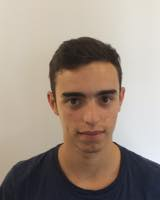
\includegraphics[height=0.8in]{Diogo} &  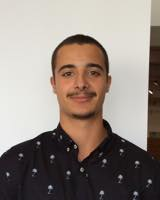
\includegraphics[height=0.8in]{Henrique} \\
	& \\
 Pedro Moreira (a82364)  &   Pedro Ferreira (a81135) \\
 
\includegraphics[height=0.8in]{PedroM} & 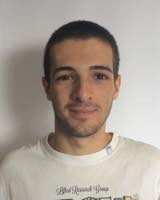
\includegraphics[height=0.8in]{PedroF} \\

\end{tabular}
\end{table}

\newpage
\tableofcontents
\newpage

\section{Introdução}
A primeira fase do projeto da UC Desenvolvimento de Sistemas de Software consistiu no desenvolvimento dos modelos de domínio, use cases e da interface com o utilizador para a aplicação ConfiguraFácil. 

Na segunda fase, desenvolvemos os diagramas de sequência, de pacotes, de implementação e de classes. Além disso, procedemos também a implementação da aplicação em si, utilizando os modelos desenhados previamente. Para tal, utilizamos DAOs para podermos fazer a conexão entre a base de dados e a aplicação em JAVA. Alterámos também alguns modelos que apresentamos na fase anterior, corrigindo para uma versão que mais se foca nos objetivos da aplicação que pretendíamos modelar.

A aplicação \textit{ConfiguraFácil} consiste numa ferramenta existente nos stands de automóveis, que permite junto dos clientes criar uma configuração para uma encomenda de um carro novo. A aplicação guia o cliente em cada fase da configuração, permitindo-lhe escolher componentes individuais ou pacotes pré-definidos. 

Da perspetiva do grupo, a aplicação apresenta os seguintes requisitos:
\begin{itemize}
	\item O cliente pode escolher a pintura, jantes e pneus, motorização e detalhes interiores e exteriores;
	\item O cliente pode também escolher um pacote pré-definido que consiste num agregado de componentes individuais;
	\item Cada componente deve ter uma designação, preço, lista de componentes incompatíveis e lista de componentes complementares;
	\item Sempre que um componente é adicionado à configuração, a aplicação deve verificar se existe alguma incompatibilidade com algum componente previamente selecionado. Se tal existir, o cliente pode optar por desistir da seleção feita ou remover o produto incompatível. Além disso, deve também verificar se é necessário instalar algum componente complementar. Caso aconteça, o cliente pode manter a opção e instalar os componentes necessários ou então desistir da seleção;
	\item Quando um pacote pré-definido é selecionado, devem ser feitas as verificações de dependência/incompatibilidade para cada um dos componentes do pacote;
	\item Deve haver descontos associados aos pacotes, ou seja, os pacotes devem ser mais baratos que a soma os preços individuais de cada um dos seus componentes;
	\item Se o cliente selecionar individualmente todos os componentes que compõem um pacote, a aplicação deve reconhecer tal pacote e aplicar o respetivo desconto;
	\item Após as escolhas básicas, como a pintura e a motorização, o cliente deve poder indicar um orçamento para a encomenda e o sistema deve propor a melhor configuração possível dentro do orçamento apresentado. Ou seja, a aplicação deve conseguir gerar uma configuração ótima dado um orçamento;
	\item Cada componente deve ter um stock associado;
	\item Sempre que chega um novo stock de componentes, o sistema deve conseguir determinar quais são os carros que podem ser produzidos;
	\item Os carros são produzidos por ordem de chegada à fila de configurações efetuadas pelos clientes.
\end{itemize}
Desta forma, procuramos cobrir todos estes requisitos, de forma a que a aplicação seja o mais completa e coesa possível. Além do referido, incluimos também as funcionalidades de registar, identificar, consultar e alterar clientes, login de funcionários (sendo que o administrador pode registar, remover ou alterar os dados destes) e as funcionalidades relativas à gestão de fábrica de encomendar stock e registar a sua entrada no sistema.

\begin{center}
\section*{1ª Fase}
\end{center}

\section{Diagrama de Domínio}
Para a aplicação que nos foi proposta e que descrevemos acima, desenvolvemos o diagrama de domínio que apresentamos de seguida:
\begin{center}
 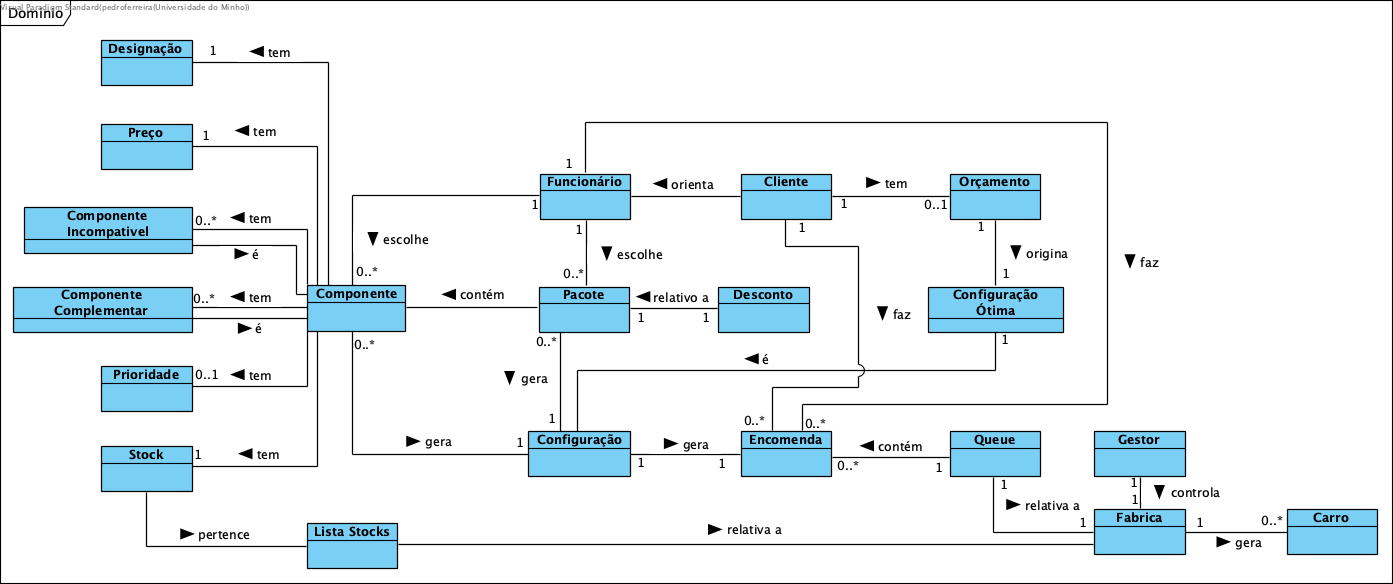
\includegraphics[width = 6.5in]{Dominio.png}
\end{center}

\newpage
\section{Diagrama de Use Cases}
\label{useCases}
Os Use Cases por nós apresentados e especificados na secção seguinte foram organizados em seis diagramas:
\begin{enumerate}
	\item Geral
		\begin{center}
 			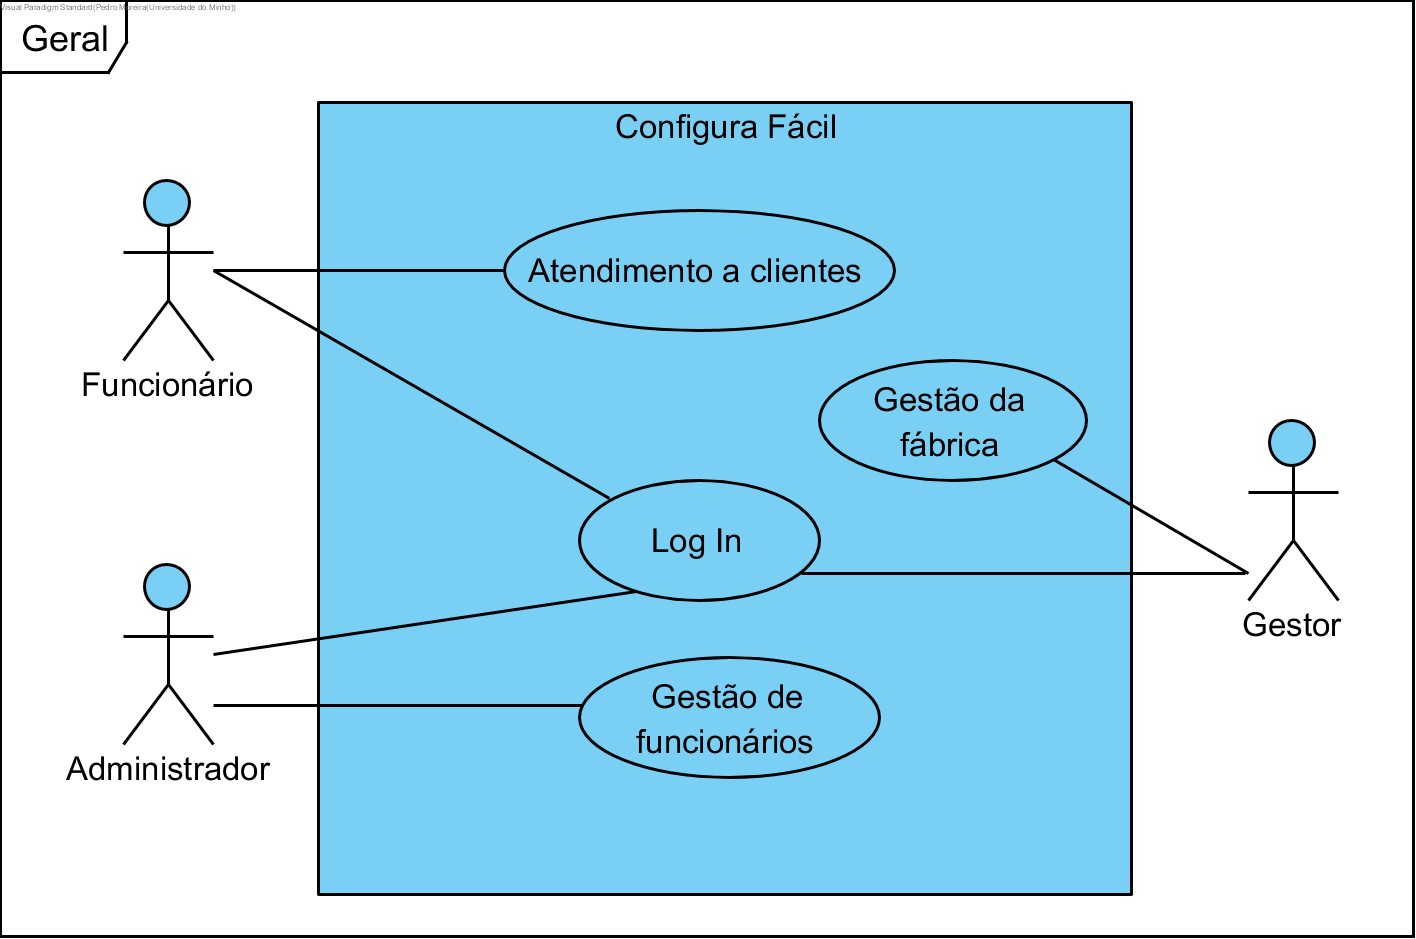
\includegraphics[]{Geral.png}
		\end{center}
	\item Gestão de Funcionários
		\begin{center}
 			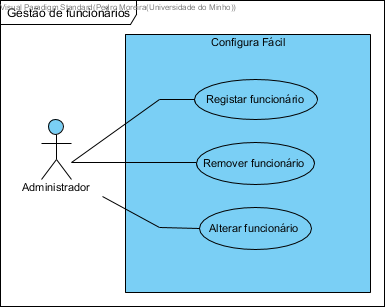
\includegraphics[]{Gestao_de_funcionarios.png}
		\end{center}\newpage
	\item Gestão de Clientes
		\begin{center}
 			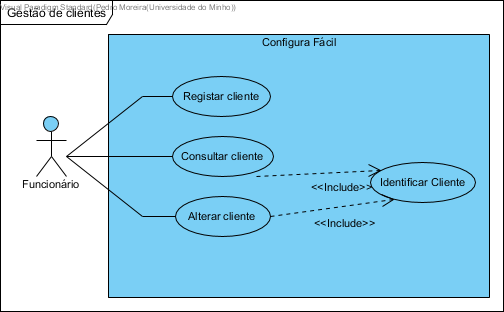
\includegraphics[]{Gestao_de_clientes.png}
		\end{center}
	\item Atendimento a Clientes
		\begin{center}
 			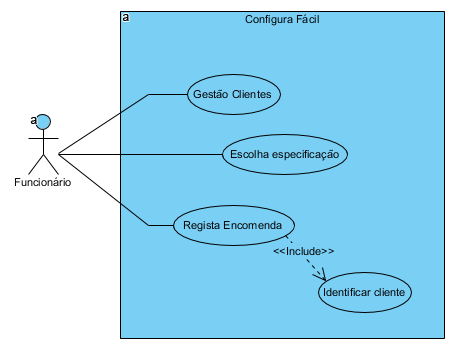
\includegraphics[]{Atendimento_a_clientes.png}
		\end{center}\newpage
	\item Escolha da Especificação
		\begin{center}
 			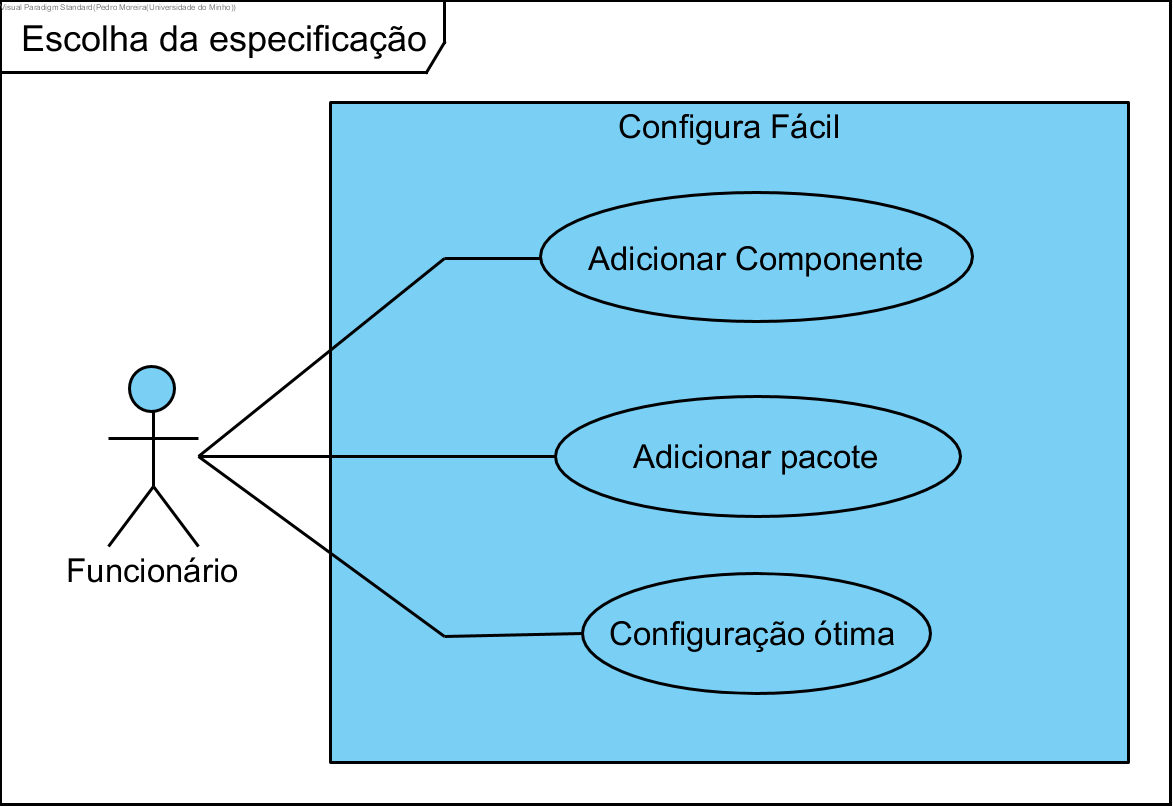
\includegraphics[]{Escolha_da_especificacao.png}
		\end{center}
	\item Gestão da Fábrica
		\begin{center}
 			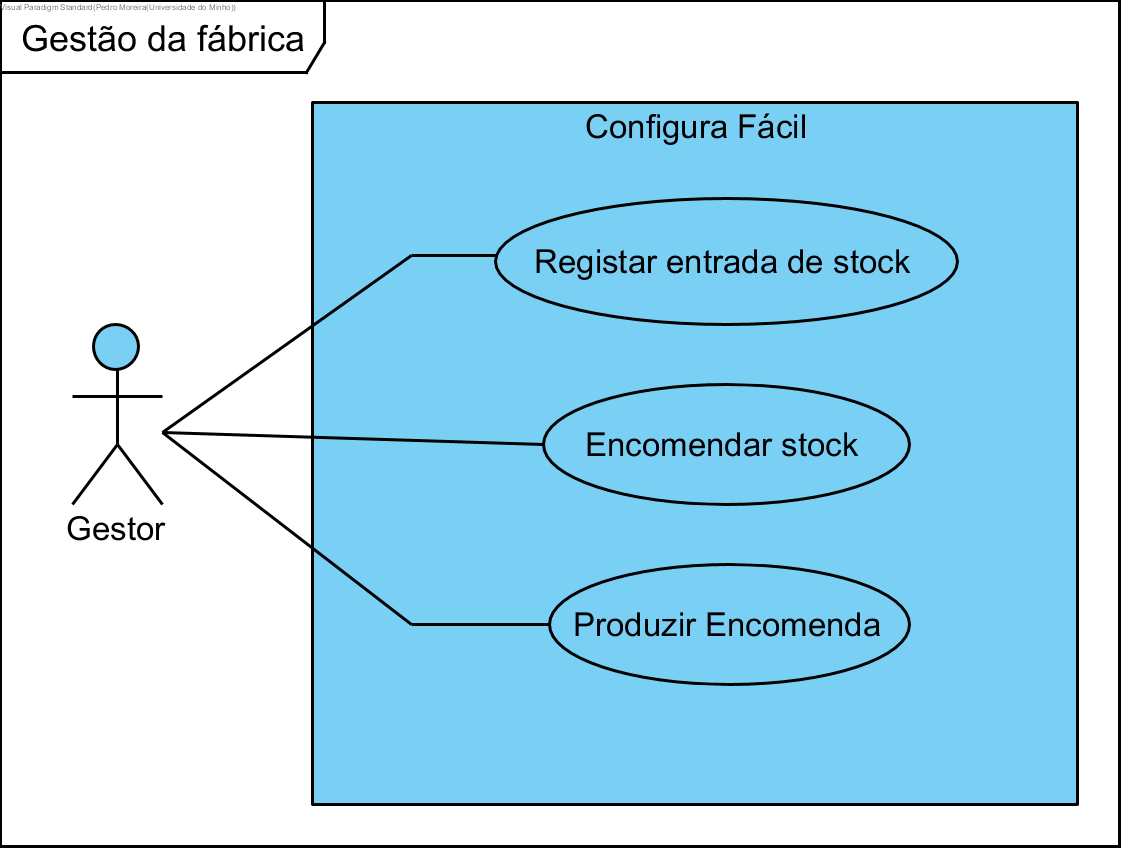
\includegraphics[]{Gestao_da_fabrica.png}
		\end{center}
\end{enumerate}

\newpage
\section{Especificação de Use Cases}
Nesta secção vamos expor as tabelas de especificação que fizemos para cada um dos Use Cases presentes nos diagramas da secção \ref{useCases}.

Para melhor organização, decidimos dividir as tabelas em Excel da especificação dos Use Cases em quatro ficheiros: 
\begin{enumerate}
	\item Login

 		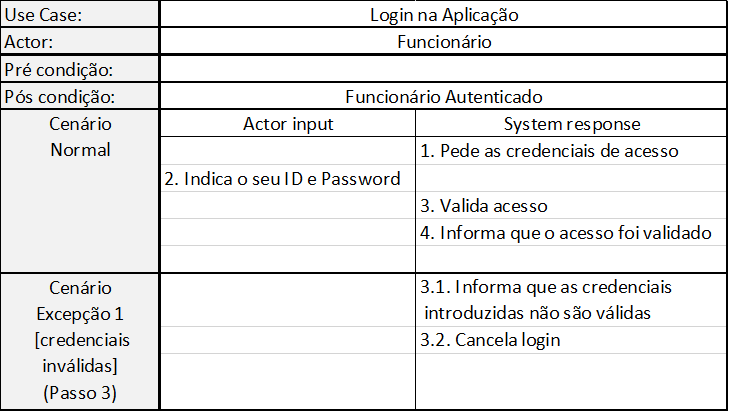
\includegraphics[width = 5in]{login.png} \newpage
	\item  Atendimento a Clientes
	\begin{center}
 		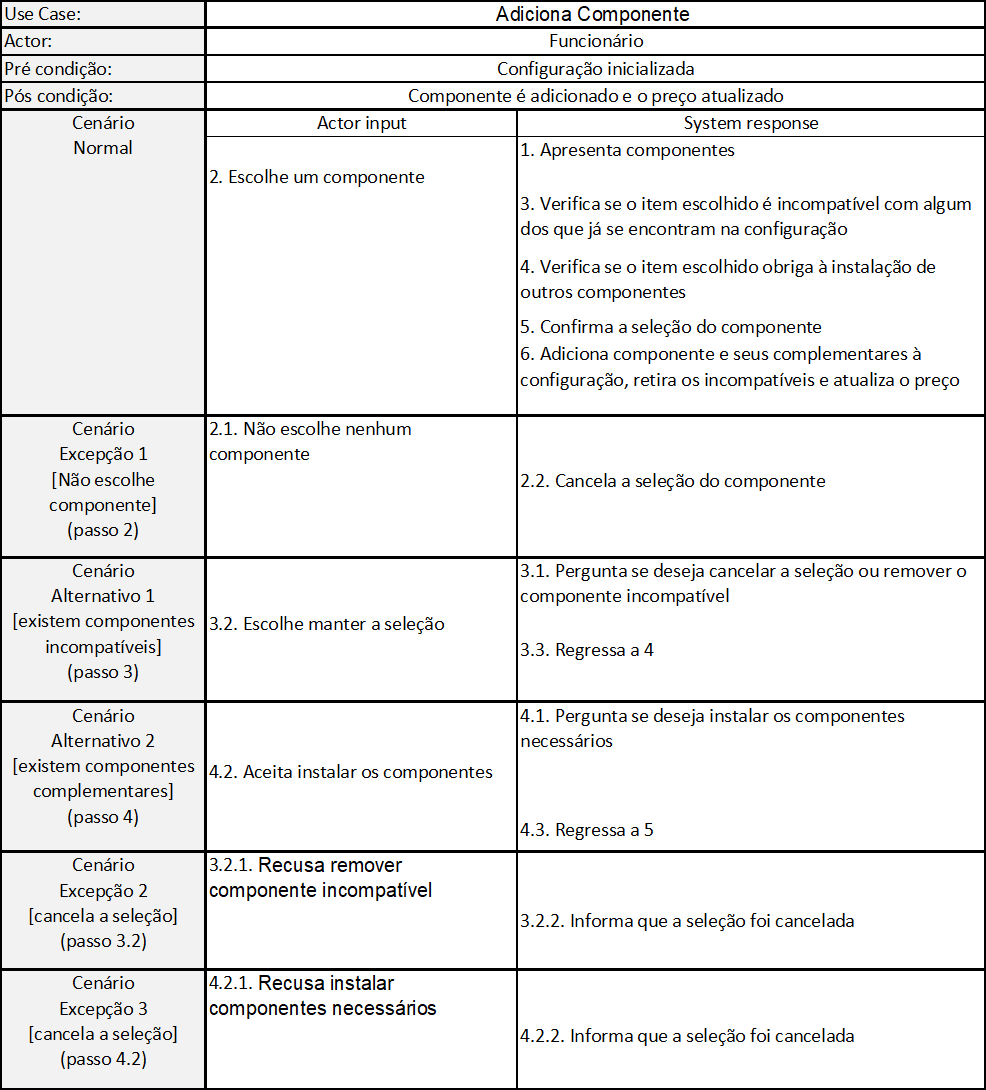
\includegraphics[width = 5in]{ac_adicionacomp.png} 
 		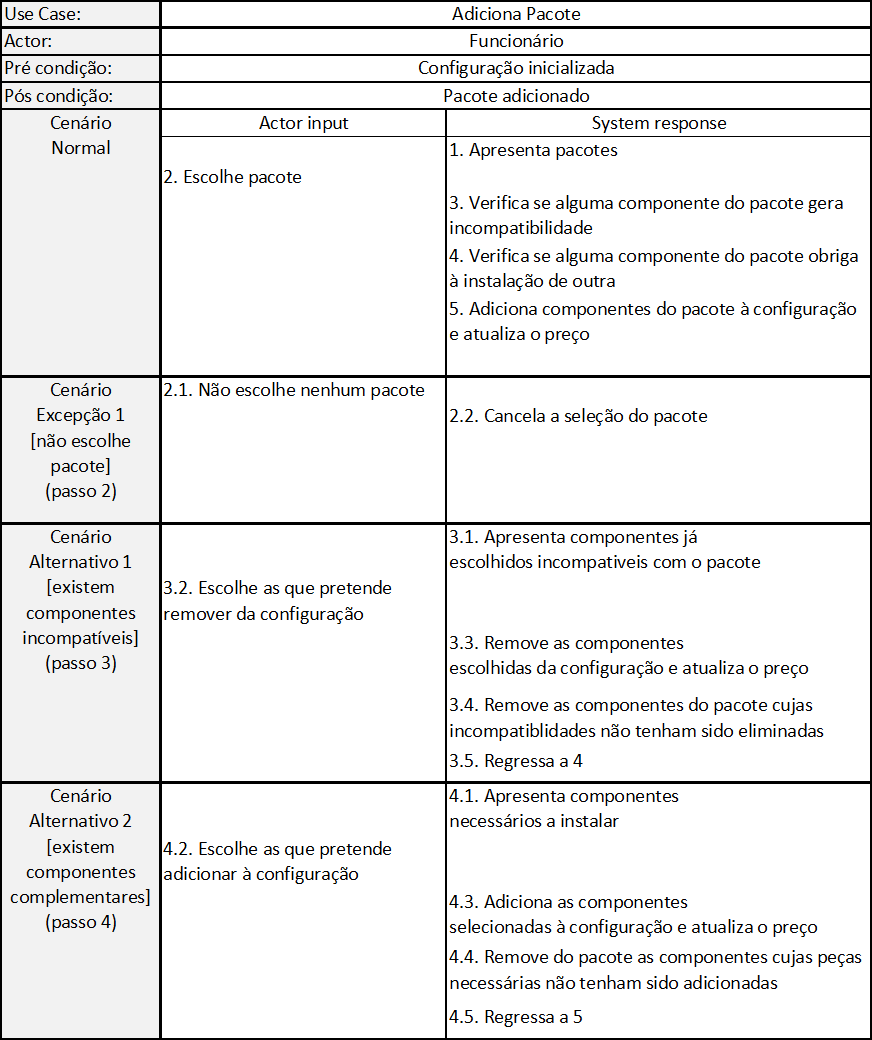
\includegraphics[width = 5in]{ac_adicionapacote.png} 
		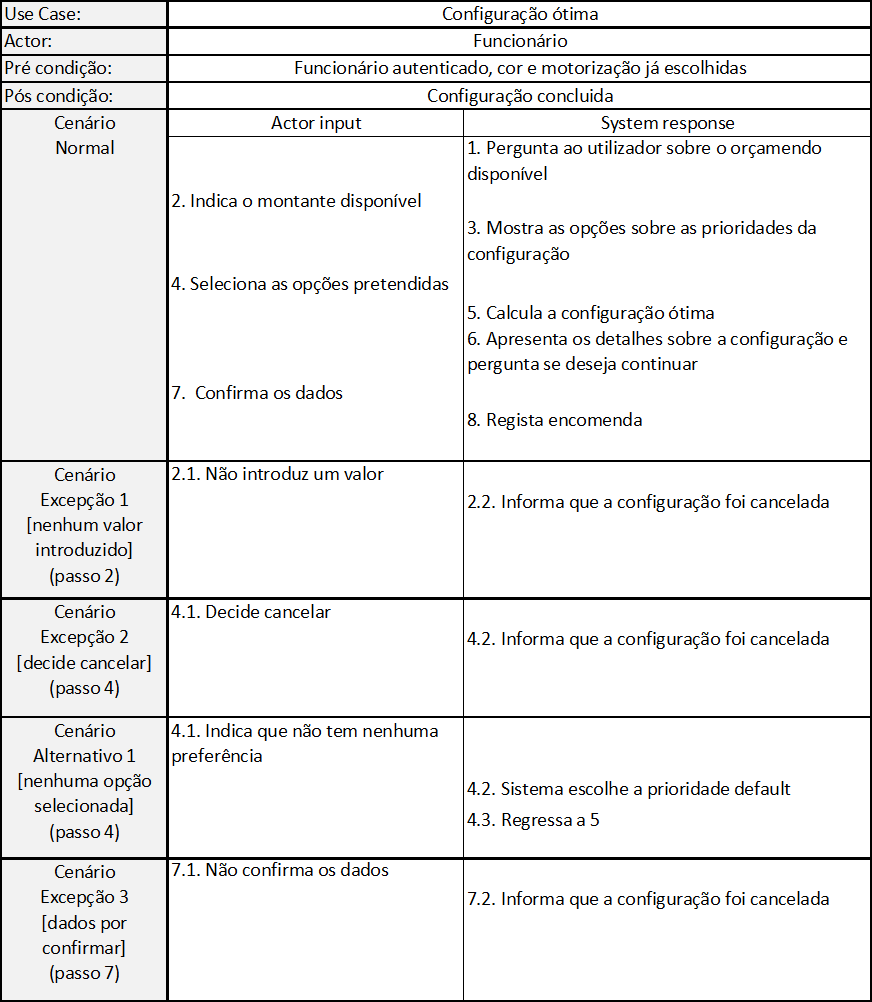
\includegraphics[width = 5in]{ac_configotima.png}
	\end{center}
	\begin{center}
		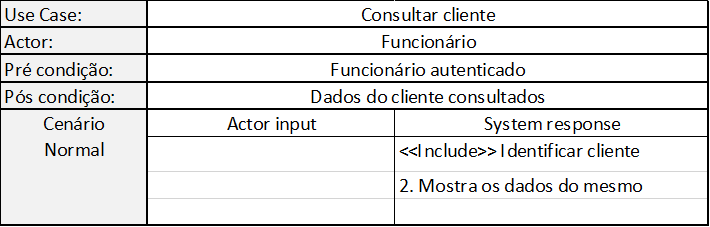
\includegraphics[width = 5in]{ac_consultarcliente.png} 
	\end{center}
	\begin{center}
		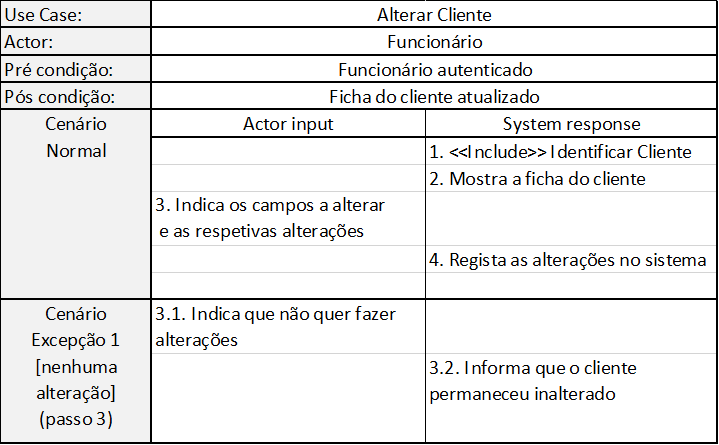
\includegraphics[width = 5in]{ac_altcliente.png}
	\end{center}
	\begin{center}
		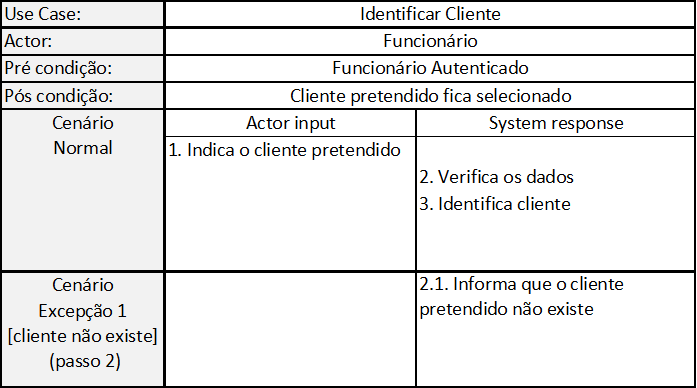
\includegraphics[width = 5in]{ac_idcliente.png}
	\end{center}
	\begin{center}
		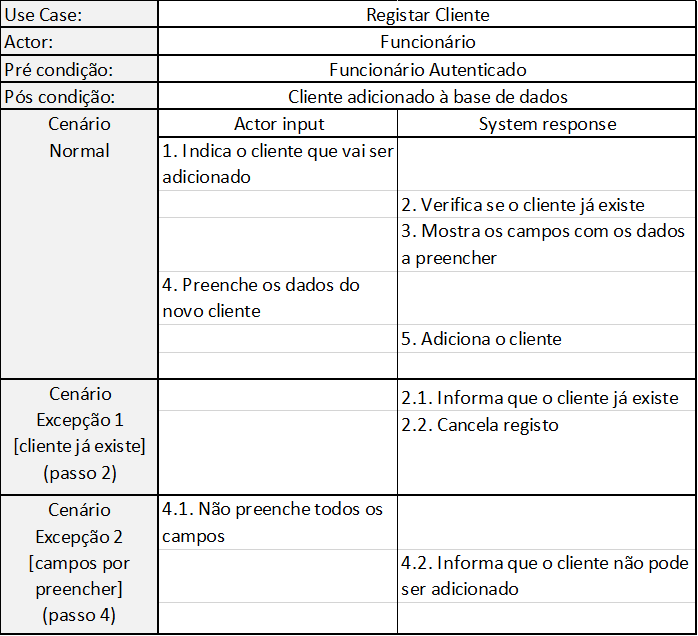
\includegraphics[width = 5in]{ac_regcliente.png}
	\end{center}
	\begin{center}
		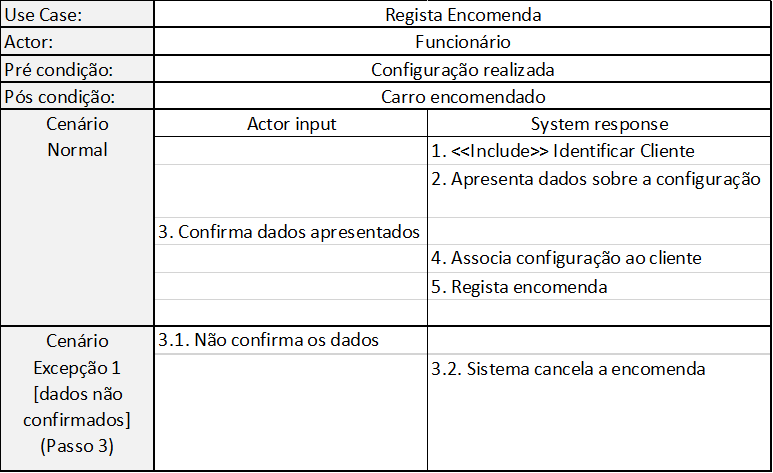
\includegraphics[width = 5in]{ac_regenc.png}
	\end{center}
	\newpage
	\item Gestão de Fábrica
	\begin{center}
		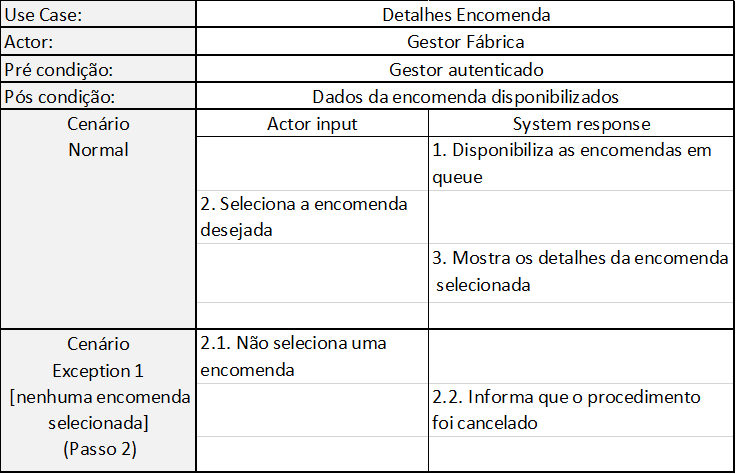
\includegraphics[width = 5in]{gf_consultarencomenda.png} 
	\end{center}
	\begin{center}
 		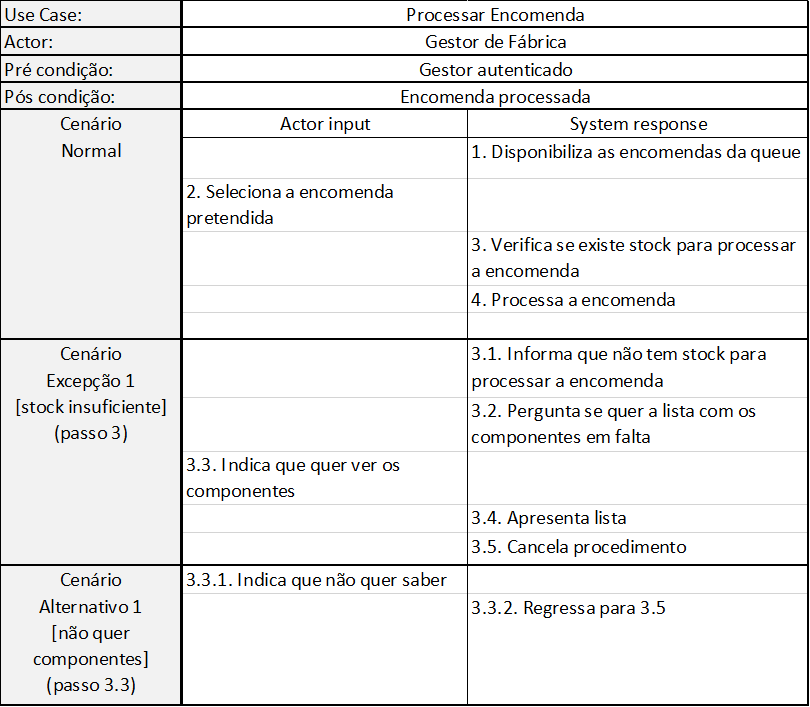
\includegraphics[width = 5in]{gf_processarencomenda.png} 
		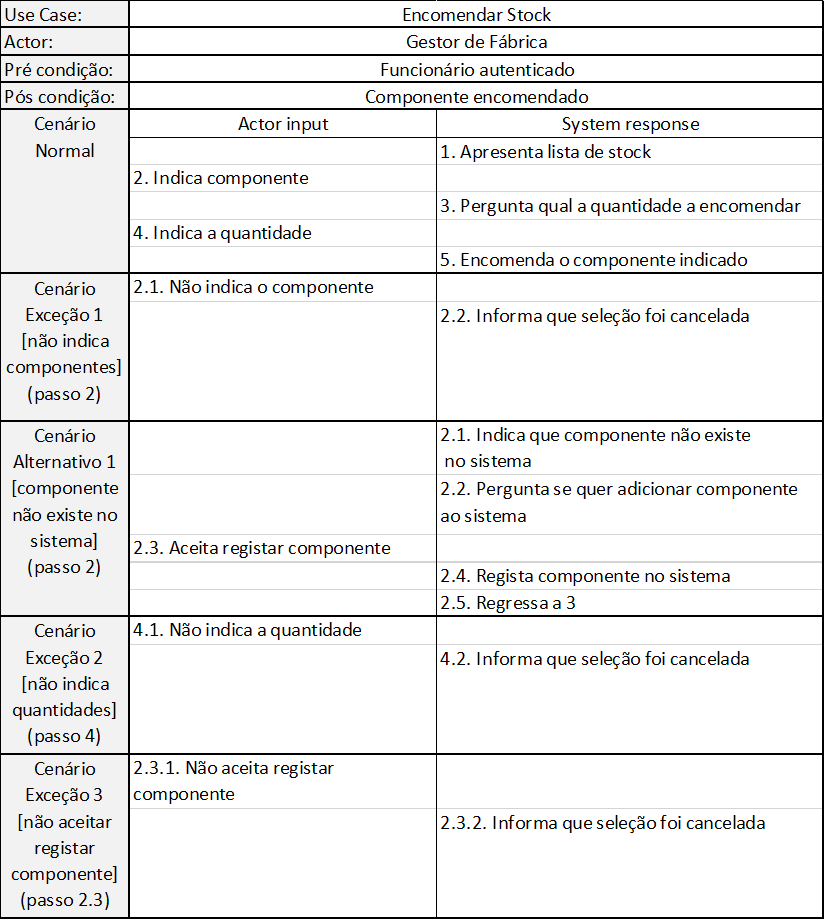
\includegraphics[width = 5in]{gf_encomendarstock.png} 
		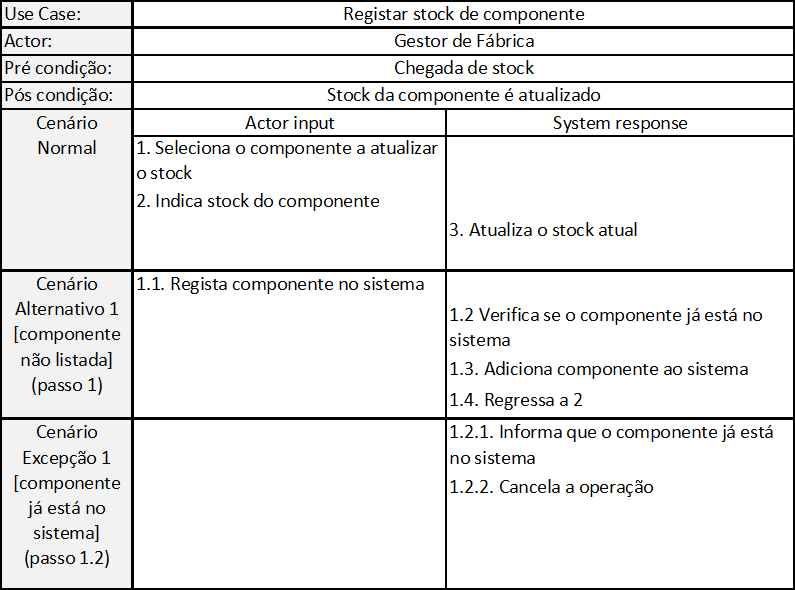
\includegraphics[width = 5in]{gf_registarstock.png}
	\end{center}
	\newpage
	\item Gestão de Funcionários
	\begin{center}
		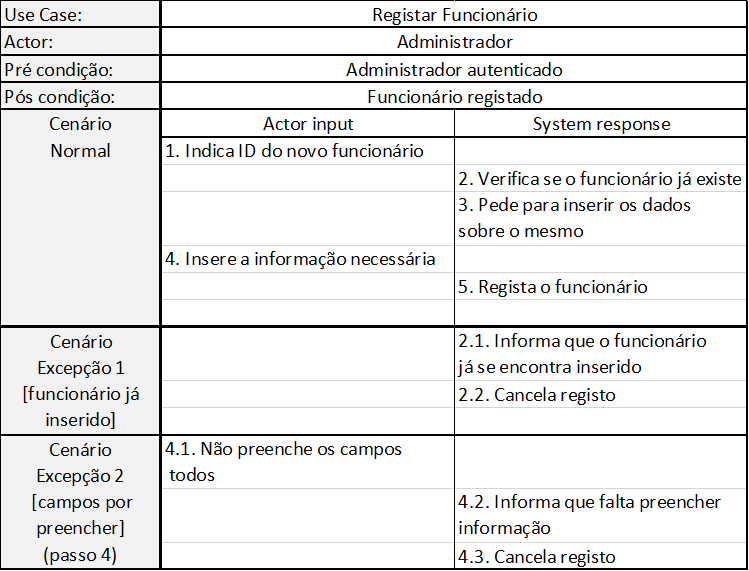
\includegraphics[width = 5in]{gfunc_registar.png} 
	\end{center}
	\begin{center}
 		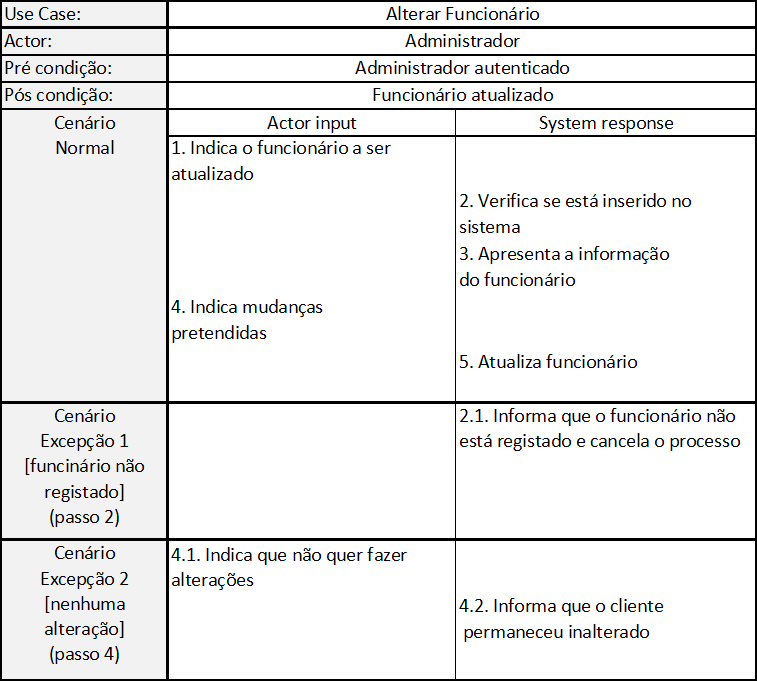
\includegraphics[width = 5in]{gfunc_alterar.png} 
	\end{center}
	\begin{center}
		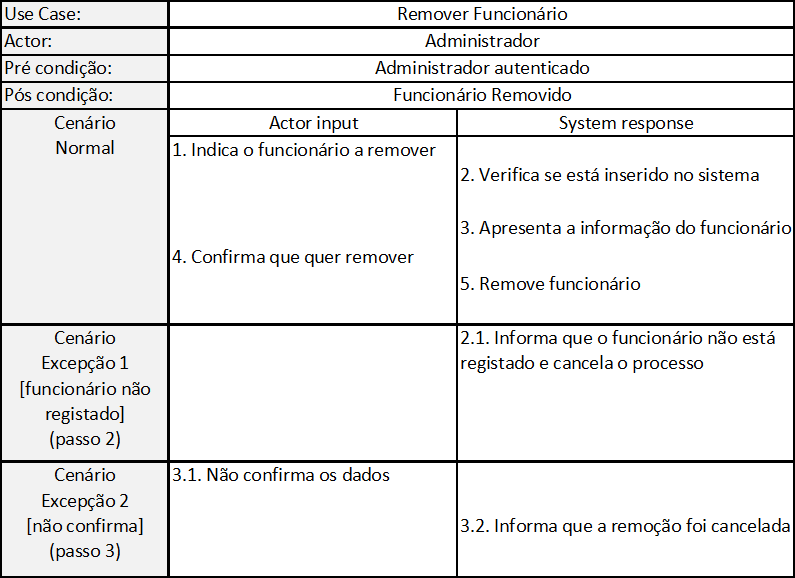
\includegraphics[width = 5in]{gfunc_remover.png}
	\end{center}
\end{enumerate}

\section{Protótipo de Interface}
O protótipo de interface para a aplicação foi feito com o \textit{Pencil}, ferramenta aconselhada pelos docentes da UC.

A página inicial do programa é a pagina de login.
\begin{center}
 	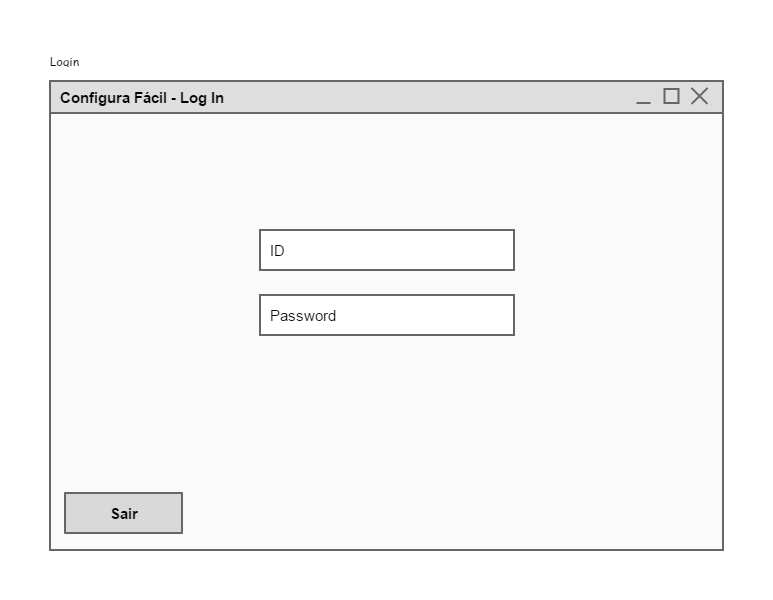
\includegraphics[width = 5in]{configura_fcil_root.png}
\end{center}

Daqui, o utilizador pode ir para uma das seguintes janelas, dependendo do seu estatuto na aplicação:

\begin{center}
 	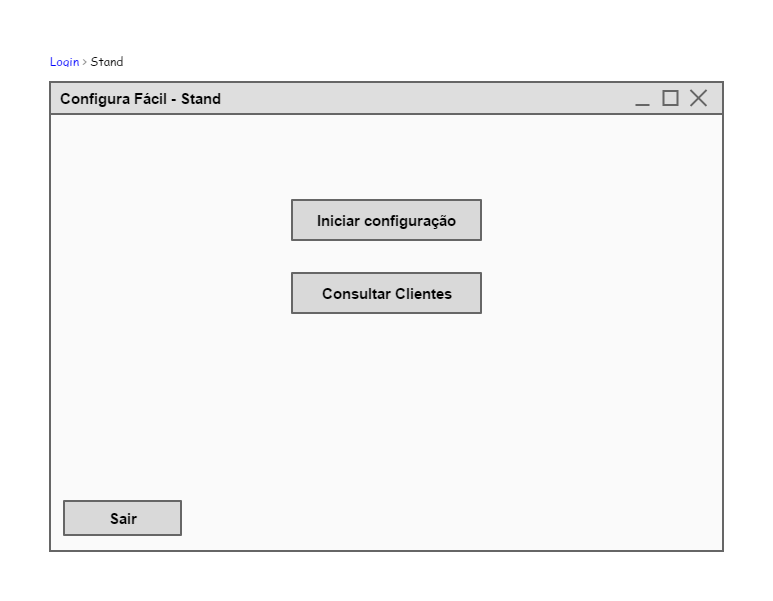
\includegraphics[width = 5.5in]{configura_fcil_stand.png}

 	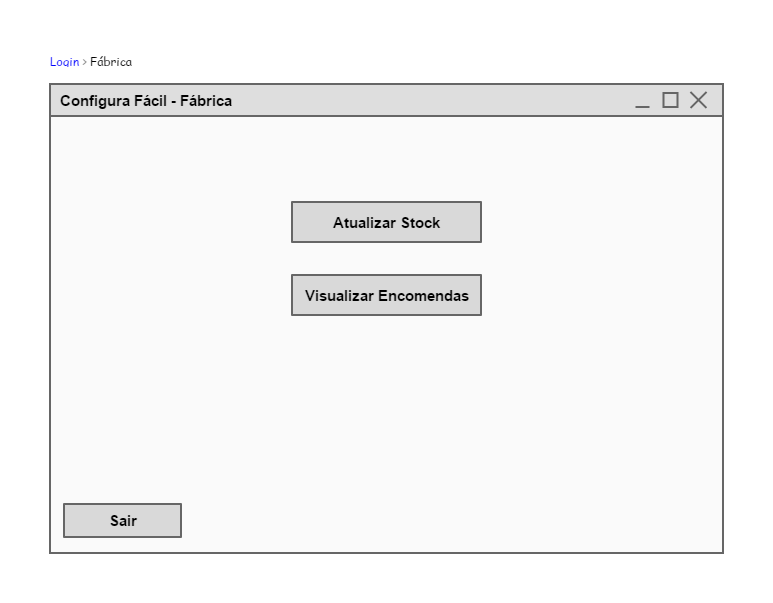
\includegraphics[width = 5.5in]{configura_fcil_fbrica.png}

 	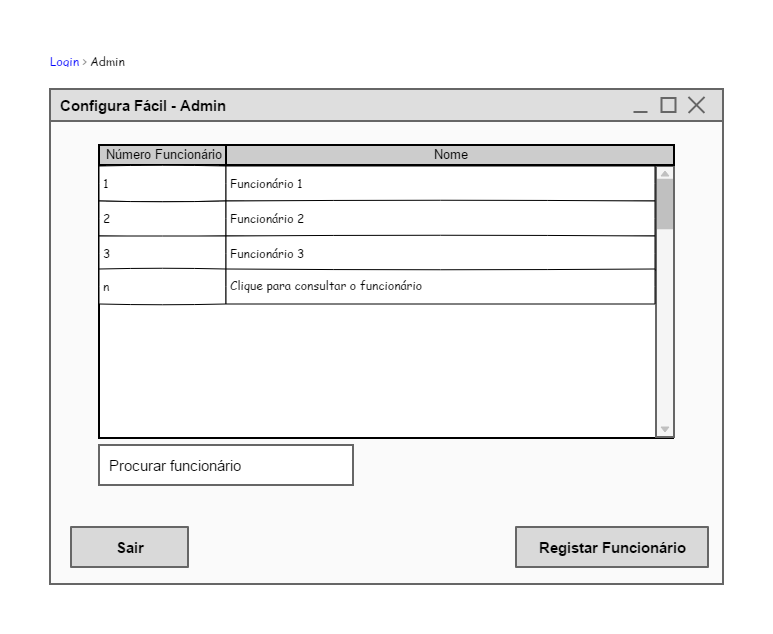
\includegraphics[width = 5.5in]{configura_fcil_admin.png}
\end{center}


A partir da janela do Stand encontramos a seguinte interface:
\begin{center}
 	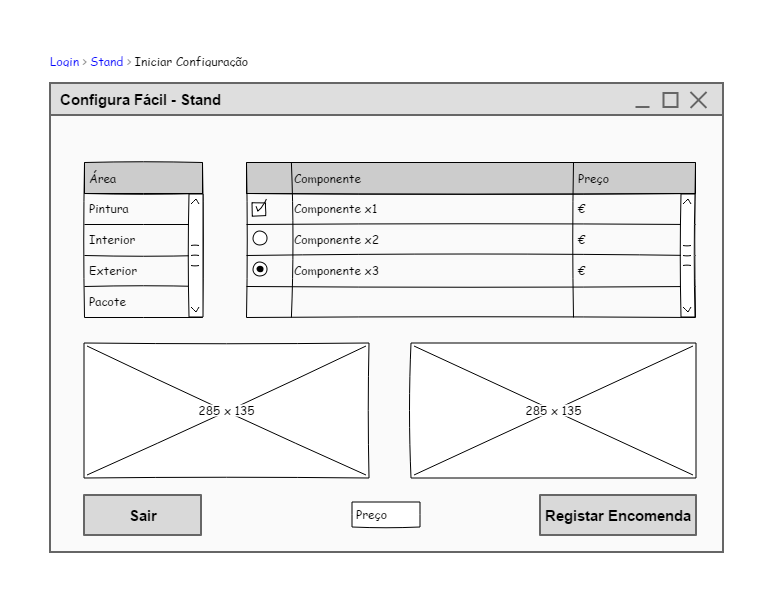
\includegraphics[width = 5in]{configurao_de_carro.png}

 	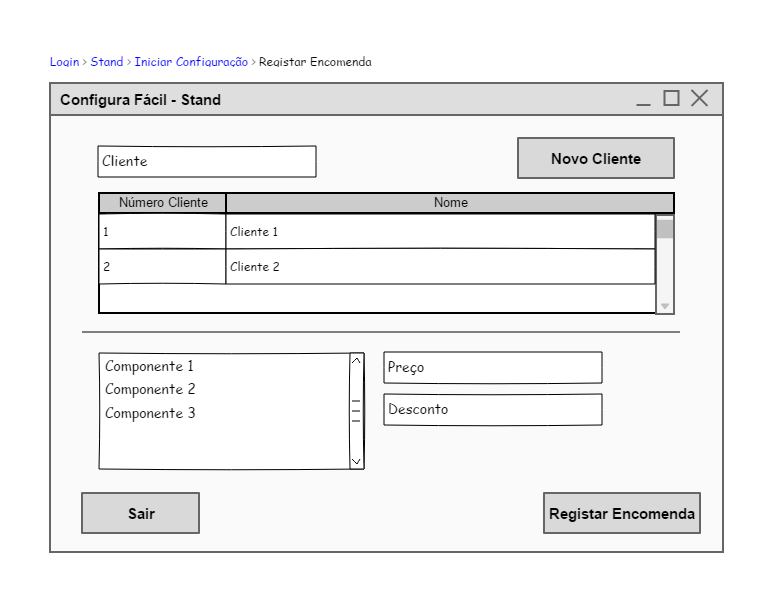
\includegraphics[width = 5.5in]{registar_encomenda.png}

 	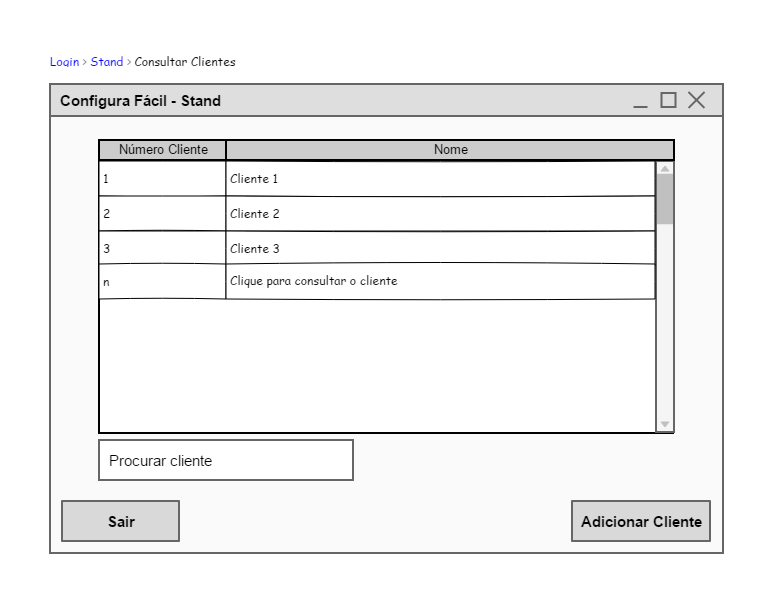
\includegraphics[width = 5.5in]{consultar_clientes.png}
	
	\begin{table}[]
		\begin{tabular}{cc}
 			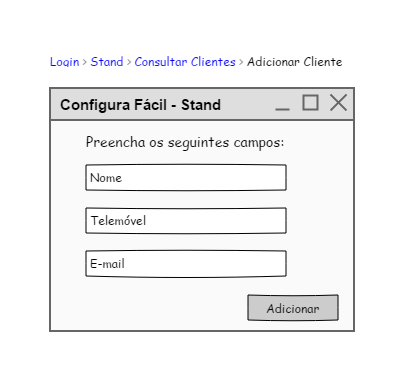
\includegraphics[width = 3in]{adicionar_cliente.png}	& 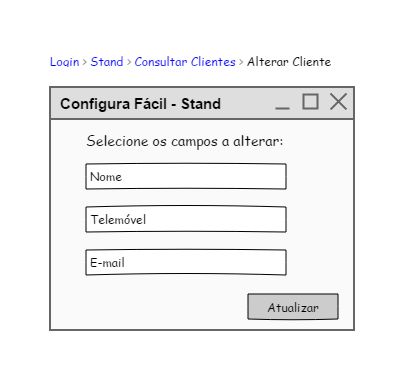
\includegraphics[width = 3in]{alterar_cliente.png}
		\end{tabular}
	\end{table}
 	 	
\end{center}

Já quando o utilizador é um gestor da fábrica, a interface gráfica que o guiará pela aplicação é a seguinte:
\begin{center}
	\begin{table}[!htbp]
		\begin{tabular}{cc}
 			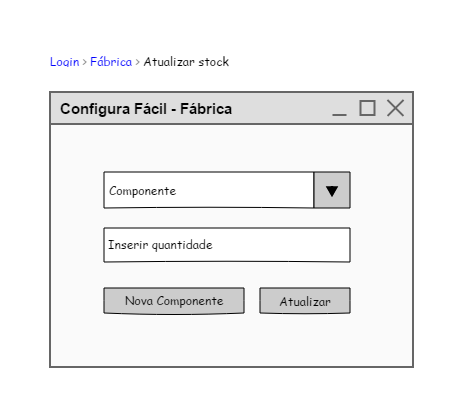
\includegraphics[width = 3in]{atualizar_stock.png} & 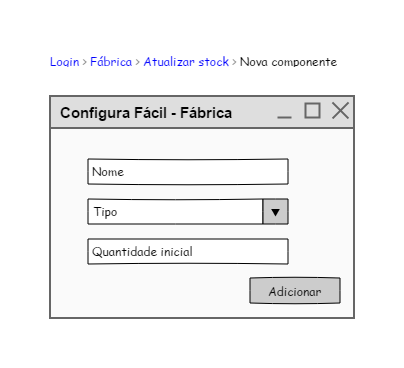
\includegraphics[width = 3in]{nova_componente.png}
		\end{tabular}
	\end{table}

 	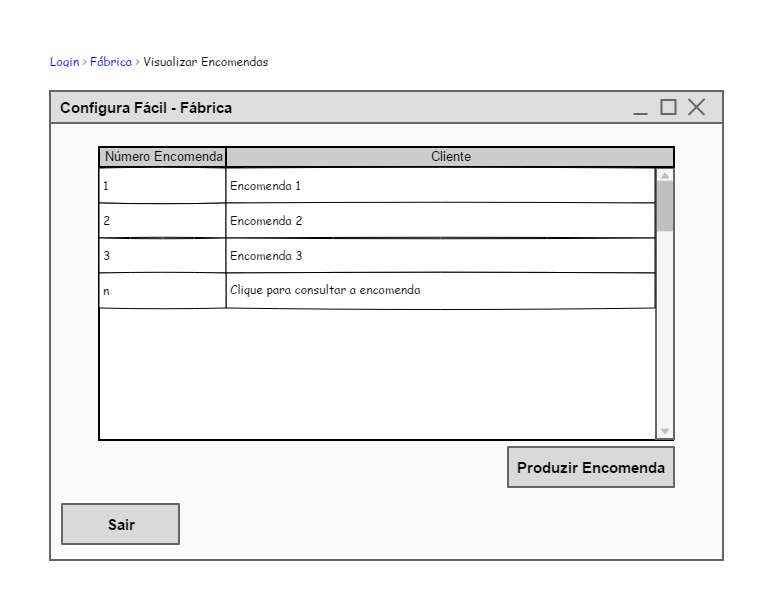
\includegraphics[width = 5.5in]{visualizar_encomendas.png}

\end{center}

Por fim, quando o funcionário faz o Login como Admistrador será esta a sua visão da aplicação:
\begin{center}
	\begin{table}[!htbp]
		\begin{tabular}{cc}
 			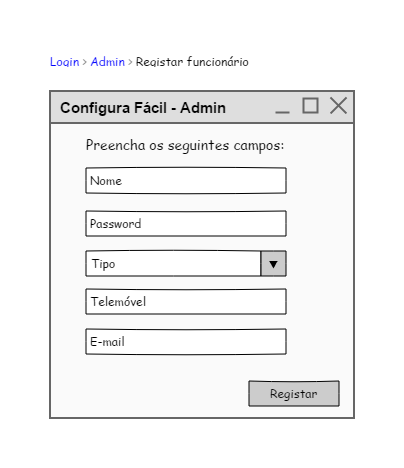
\includegraphics[width = 3in]{registar_funcionrio.png} & 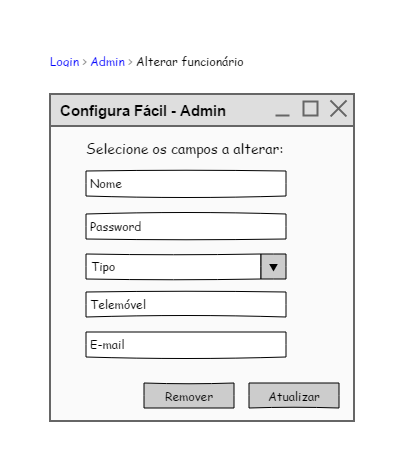
\includegraphics[width = 3in]{alterar_funcionrio.png}
		\end{tabular}
	\end{table}

\end{center}


\section{Diagrama de Máquinas de Estado}
O diagrama de Máquinas de Estado relativo à interface do programa é o seguinte:
	\begin{center}
		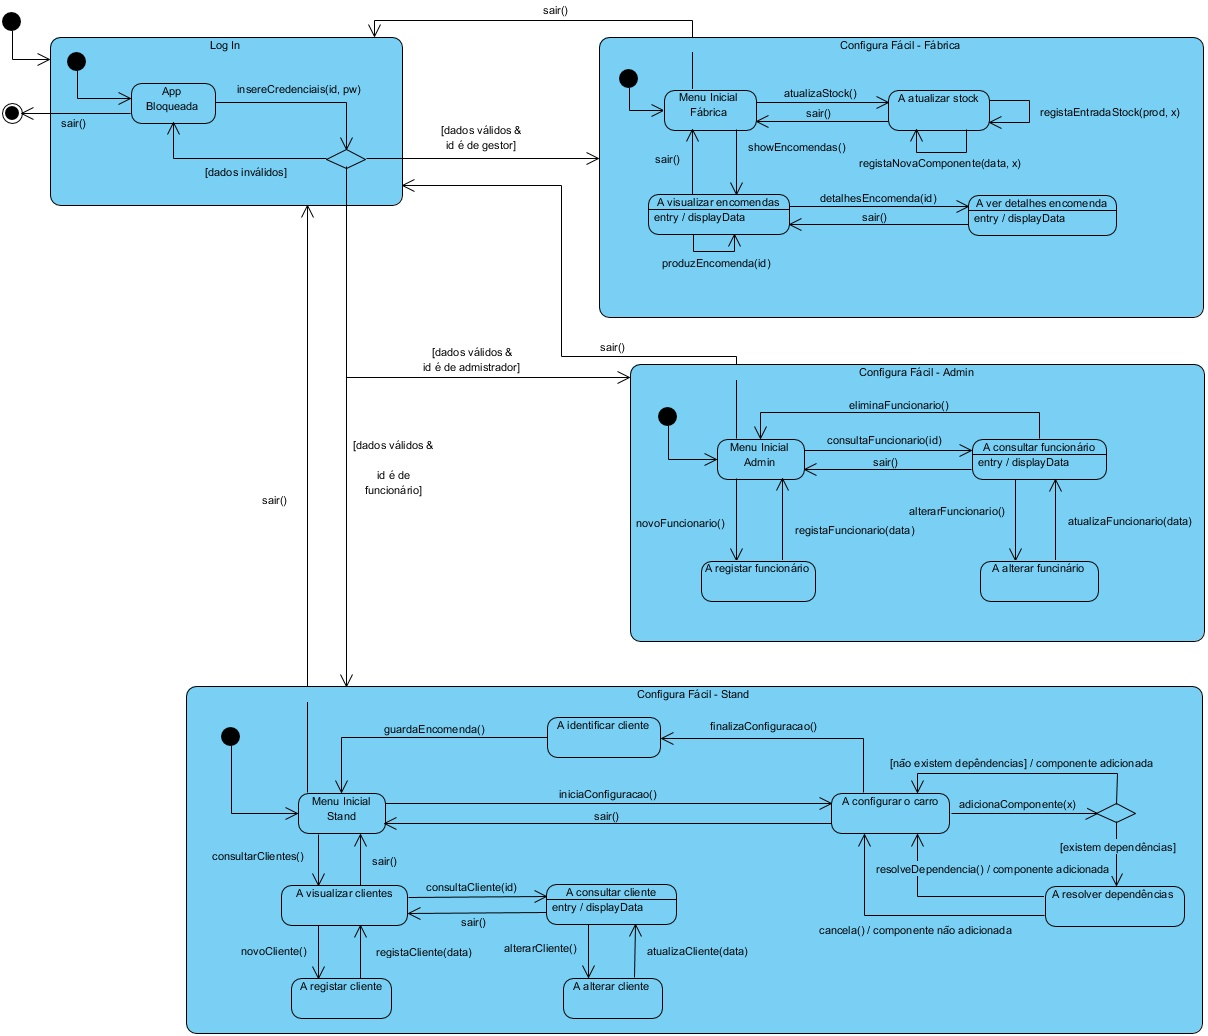
\includegraphics[width = 6in]{Maquina_de_Estado.jpg}
	\end{center}
	
\newpage

\begin{center}
\section*{2ª Fase}
\end{center}

\section{Diagramas de Sequência de Sistema}
A segunda fase do projeto principiou com a modelação dos diagramas de sequência, partindo da especificação dos Use Cases feita na fase anterior. Assim sendo, temos os seguintes diagramas:

\begin{enumerate}
	\item Adiciona Componente
		\begin{center}
 			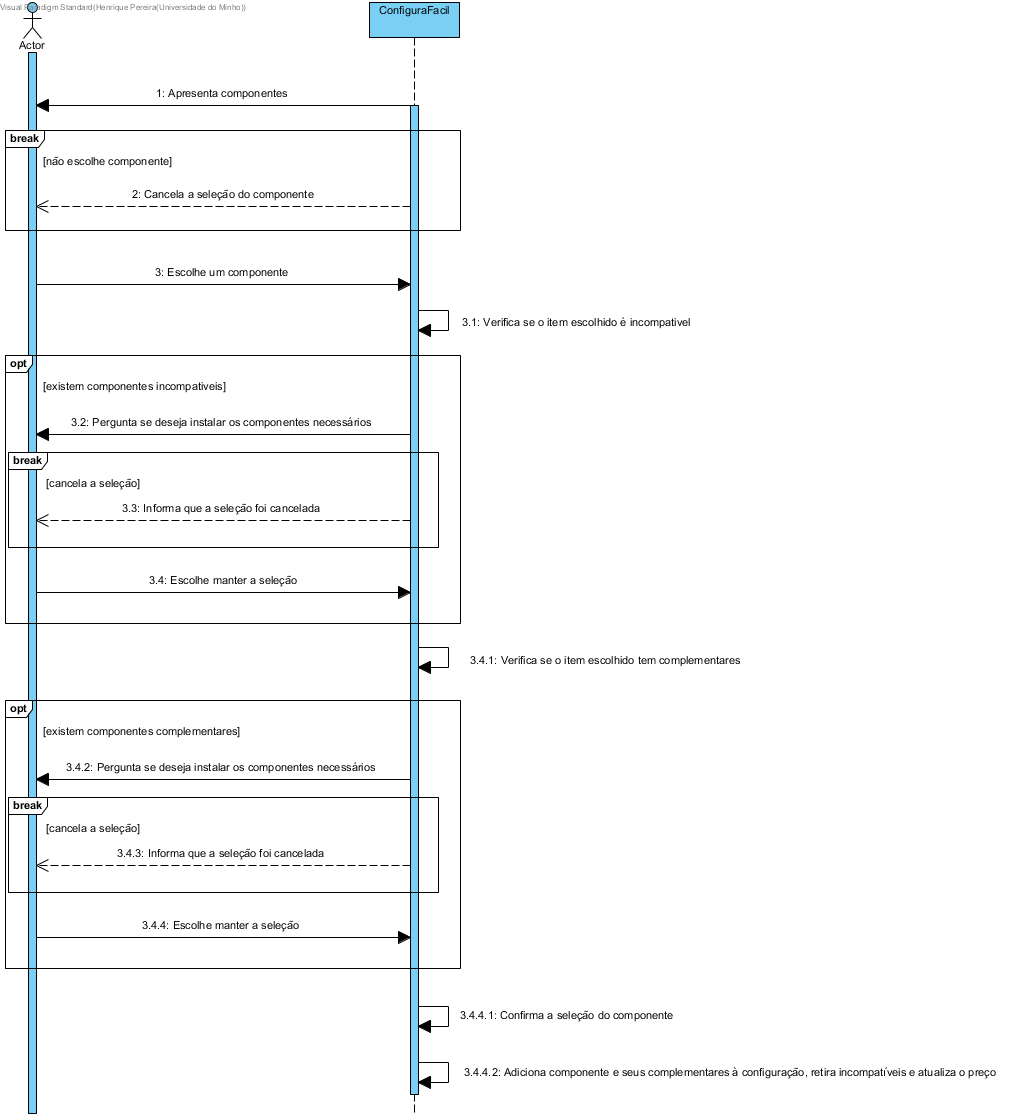
\includegraphics[width = 6in]{dss_adiciona_componente.png}
		\end{center}
	\item Adiciona Pacote
		\begin{center}
 			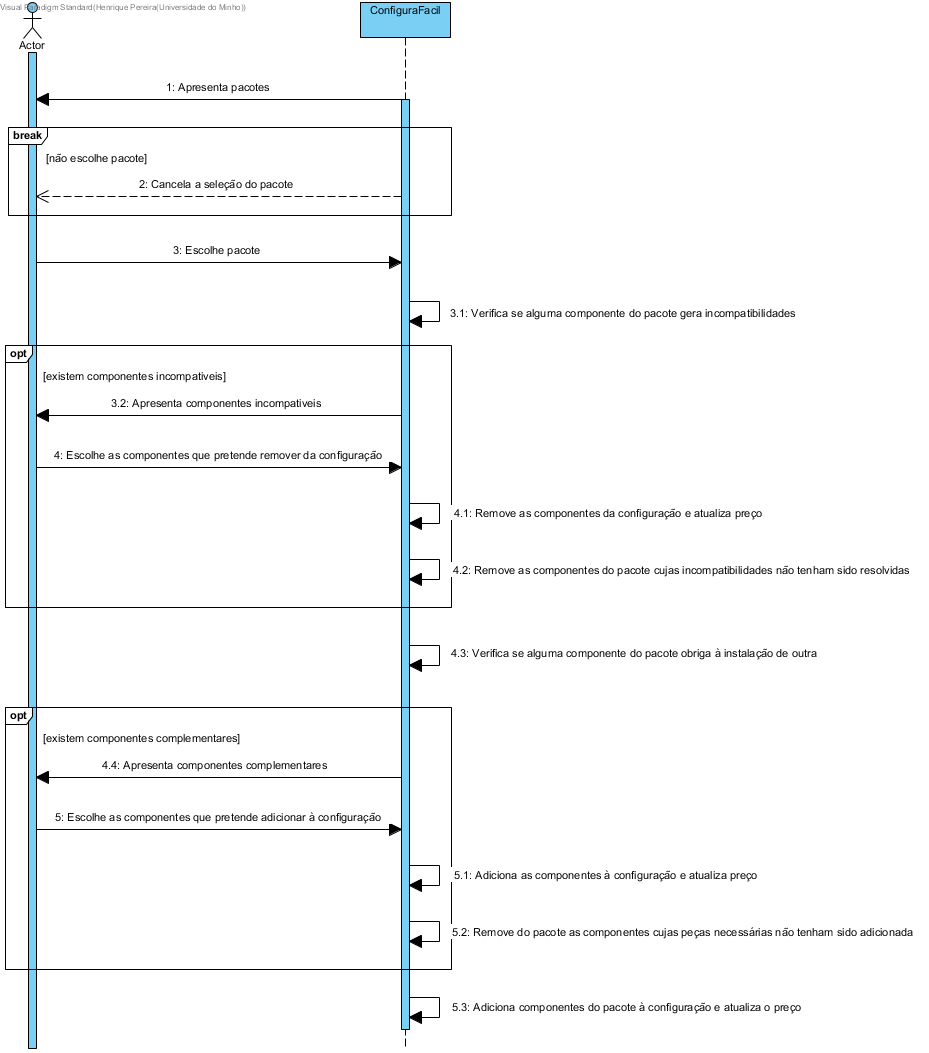
\includegraphics[width = 6in]{dss_adiciona_pacote.png}
		\end{center}\newpage
	\item Alterar Cliente
		\begin{center}
 			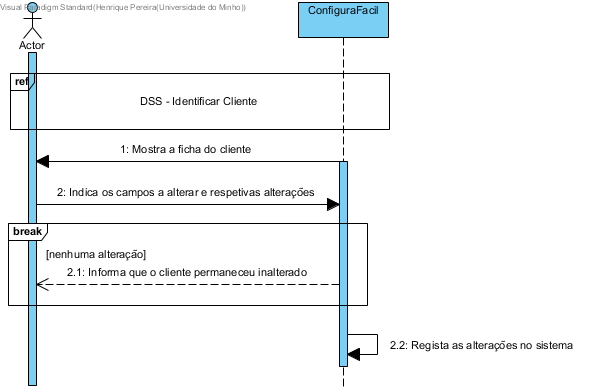
\includegraphics[width = 6in]{dss_alterar_cliente.png}
		\end{center}
	\item Alterar Funcionário
		\begin{center}
 			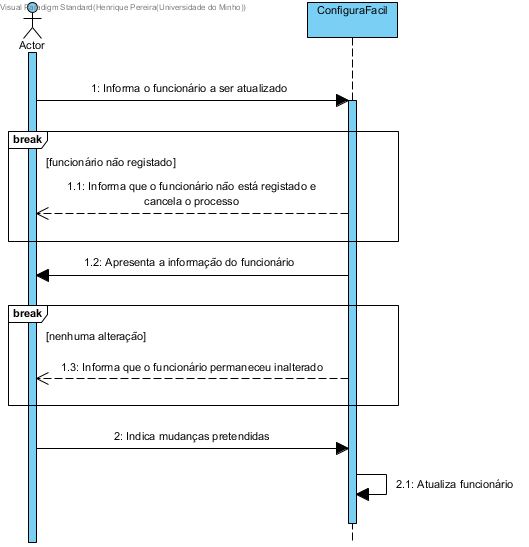
\includegraphics[width = 6in]{dss_alterar_funcionario.png}
		\end{center}\newpage
	\item Configuração Ótima
		\begin{center}
 			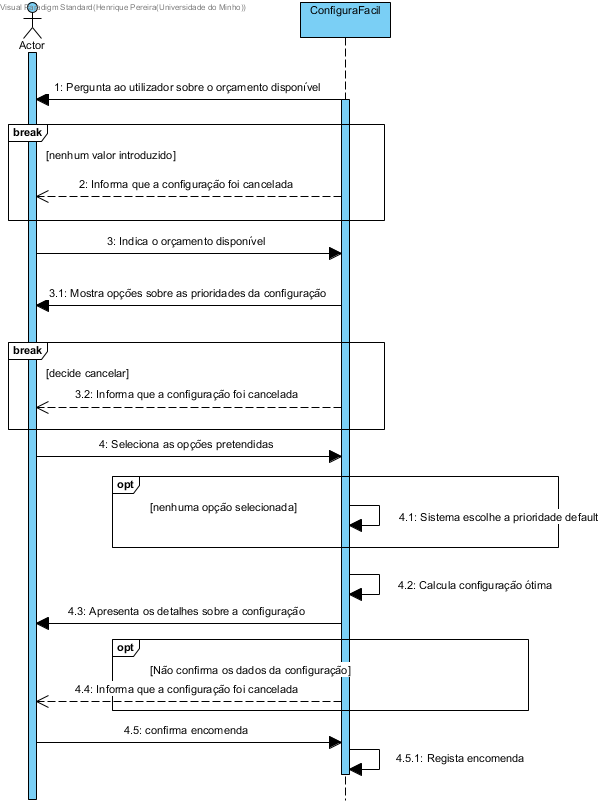
\includegraphics[width = 6in]{dss_configuracao_otima.png}
		\end{center}
	\item Consultar Cliente
		\begin{center}
 			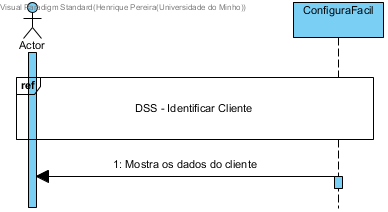
\includegraphics[width = 6in]{dss_consultar_cliente.png}
		\end{center}
	\item Consultar Encomenda
		\begin{center}
 			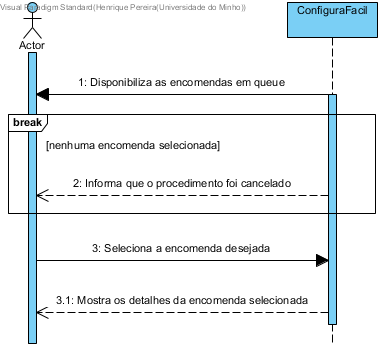
\includegraphics[width = 6in]{dss_consultar_encomenda.png}
		\end{center}
	\item Encomendar Stock
		\begin{center}
 			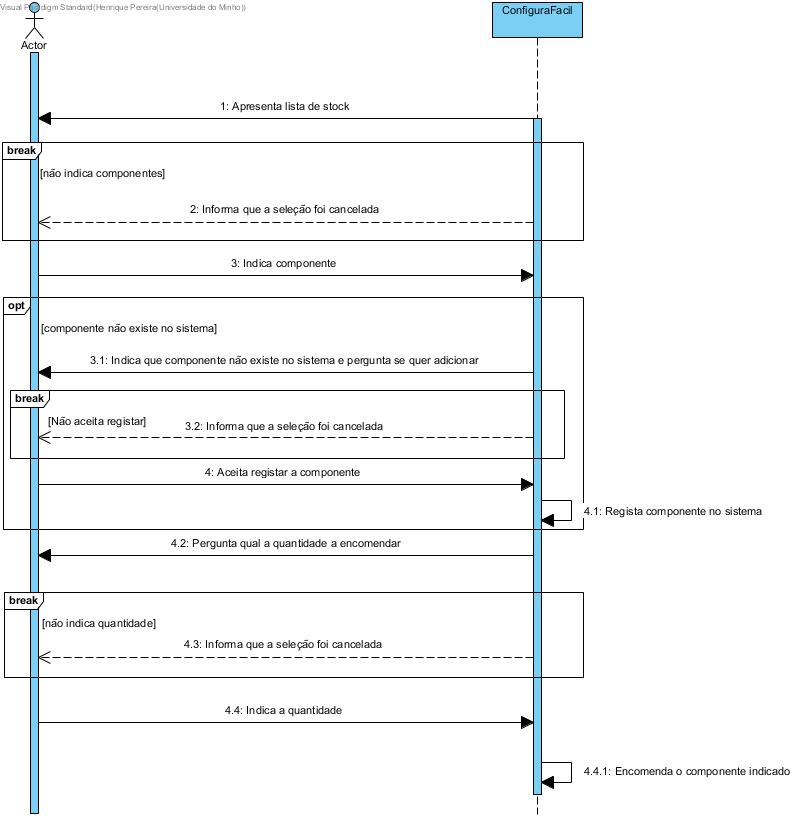
\includegraphics[width = 6in]{dss_encomendar_stock.png}
		\end{center}
	\item Identificar Cliente
		\begin{center}
 			\includegraphics[width = 6in]{dss_identificar_cliente.png}
		\end{center}
	\item Login
		\begin{center}
 			\includegraphics[width = 6in]{dss_login.png}
		\end{center}
	\item Processa Encomenda
		\begin{center}
 			\includegraphics[width = 6in]{dss_processa_encomenda.png}
		\end{center}
	\item Registar Cliente
		\begin{center}
 			\includegraphics[width = 6in]{dss_registar_cliente.png}
		\end{center}
	\item Registar Encomenda
		\begin{center}
 			\includegraphics[width = 6in]{dss_registar_encomenda.png}
		\end{center}
	\item Registar Funcionário
		\begin{center}
 			\includegraphics[width = 6in]{dss_registar_funcionario.png}
		\end{center}
	\item Registar Stock de Componente
		\begin{center}
 			\includegraphics[width = 6in]{dss_registar_stock.png}
		\end{center}
	\item Remover Funcionário
		\begin{center}
 			\includegraphics[width = 6in]{dss_remover_funcionario.png}
		\end{center}
\end{enumerate}

\section{Diagramas de Sequência com Subsistemas}
O passo seguinte foi, partindo dos diagramas de sequência e conhecendo agora os subsistemas existentes, modelar os diagramas de sequência de subsistema, para depois podemos proseguir com os diagramas de implementação.

Ora, temos então o seguinte:
\begin{enumerate}
	\item Adiciona Componente
		\begin{center}
 			\includegraphics[width = 6in]{dsss_adiciona_componente.png}
		\end{center}
	\item Adiciona Pacote
		\begin{center}
 			\includegraphics[width = 6in]{dsss_adiciona_pacote.png}
		\end{center}\newpage
	\item Alterar Cliente
		\begin{center}
 			\includegraphics[width = 6in]{dsss_alterar_cliente.png}
		\end{center}
	\item Alterar Funcionário
		\begin{center}
 			\includegraphics[width = 6in]{dsss_alterar_funcionario.png}
		\end{center}\newpage
	\item Configuração Ótima
		\begin{center}
 			\includegraphics[width = 6in]{dsss_configuracao_otima.png}
		\end{center}
	\item Consultar Cliente
		\begin{center}
 			\includegraphics[width = 6in]{dsss_consultar_cliente.png}
		\end{center}
	\item Consultar Encomenda
		\begin{center}
 			\includegraphics[width = 6in]{dsss_consultar_encomenda.png}
		\end{center}
	\item Encomendar Stock
		\begin{center}
 			\includegraphics[width = 6in]{dsss_encomendar_stock.png}
		\end{center}
	\item Identificar Cliente
		\begin{center}
 			\includegraphics[width = 6in]{dsss_identificar_cliente.png}
		\end{center}
	\item Login
		\begin{center}
 			\includegraphics[width = 6in]{dsss_login.png}
		\end{center}
	\item Processa Encomenda
		\begin{center}
 			\includegraphics[width = 6in]{dsss_processa_encomenda.png}
		\end{center}
	\item Registar Cliente
		\begin{center}
 			\includegraphics[width = 6in]{dsss_registar_cliente.png}
		\end{center}
	\item Registar Encomenda
		\begin{center}
 			\includegraphics[width = 6in]{dsss_registar_encomenda.png}
		\end{center}
	\item Registar Funcionário
		\begin{center}
 			\includegraphics[width = 6in]{dsss_registar_funcionario.png}
		\end{center}
	\item Registar Stock de Componente
		\begin{center}
 			\includegraphics[width = 6in]{dsss_registar_stock.png}
		\end{center}
	\item Remover Funcionário
		\begin{center}
 			\includegraphics[width = 6in]{dsss_remover_funcionario.png}
		\end{center}
\end{enumerate}

\section{Diagrama de Packages}
De forma a organizarmos melhor a aplicação, dividimos o sistema geral em quatro subsistemas: o Facade (que corresponde à ConfiguraFácil), o gContas, o gConfig e o gFabrica. Como tal, construímos o seguinte diagrama de pacotes:
\begin{center}
 	\includegraphics[width=6in]{pacotes.jpg}
\end{center}

\section{Diagrama de Classe com Estruturas de Dados e com ORM}
Partindo do Modelo de Domínio e dos diagramas de sequência de implementação, podemos definir o Diagrama de Classes:
\begin{center}
 	\includegraphics[width=6in]{Classes.png}
\end{center}

O passo seguinte foi, tendo em conta o ORM, decidir quais as classes que deveriam persistir. Assim, pela nossa análise, selecionamos as seguintes classes: Cliente, Funcionário, Encomenda, Componente, Pacote e Stock. Deste modo, obtivemos o seguinte diagrama de classes, já com as estruturas de dados e com ORM:
\begin{center}
 	\includegraphics[width=6in]{ClassesDAO.png}
\end{center}


\section{Diagramas de Sequência de Implementação}
Como foi referido, podemos agora desenhar os diagramas de sequência de implementação. Com estes definidos, podemos começar a escrever o código para a aplicação, partindo de uma base bastante consistente.

Para tal, modelamos os ditos diagramas da seguinte maneira:
\begin{enumerate}
	\item Adiciona Componente
		\begin{center}
 			\includegraphics[width = 6in]{dsi_adicionar_componente.png}
		\end{center}
	\item Adiciona Pacote
		\begin{center}
 			\includegraphics[width = 6in]{dsi_adicionar_pacote.png}
		\end{center}\newpage
	\item Alterar Cliente
		\begin{center}
 			\includegraphics[width = 6in]{dsi_alterar_cliente.png}
		\end{center}
	\item Alterar Funcionário
		\begin{center}
 			\includegraphics[width = 6in]{dsi_alterar_funcionario.png}
		\end{center}\newpage
	\item Configuração Ótima
		\begin{center}
 			\includegraphics[width = 6in]{dsi_configuracao_otima.png}
		\end{center}
	\item Consultar Cliente
		\begin{center}
 			\includegraphics[width = 6in]{dsi_consultar_cliente.png}
		\end{center}
	\item Consultar Encomenda
		\begin{center}
 			\includegraphics[width = 6in]{dsi_consultar_encomenda.png}
		\end{center}
	\item Encomendar Stock
		\begin{center}
 			\includegraphics[width = 6in]{dsi_encomendar_stock.png}
		\end{center}
	\item Identificar Cliente
		\begin{center}
 			\includegraphics[width = 6in]{dsi_identificar_cliente.png}
		\end{center}
	\item Login
		\begin{center}
 			\includegraphics[width = 6in]{dsi_login.png}
		\end{center}
	\item Processa Encomenda
		\begin{center}
 			\includegraphics[width = 6in]{dsi_processar_encomenda.png}
		\end{center}
	\item Registar Cliente
		\begin{center}
 			\includegraphics[width = 6in]{dsi_registar_cliente.png}
		\end{center}
	\item Registar Encomenda
		\begin{center}
 			\includegraphics[width = 6in]{dsi_registar_encomenda.png}
		\end{center}
	\item Registar Funcionário
		\begin{center}
 			\includegraphics[width = 6in]{dsi_registar_funcionario.png}
		\end{center}
	\item Registar Stock de Componente
		\begin{center}
 			\includegraphics[width = 6in]{dsi_registar_stock.png}
		\end{center}
	\item Remover Funcionário
		\begin{center}
 			\includegraphics[width = 6in]{dsi_remover_funcionario.png}
		\end{center}
\end{enumerate}

Tendo em conta os DAOs, os diagramas de sequência de implementação alterar-se-ão da seguinte maneira:
\begin{enumerate}
	\item Adiciona Componente
		\begin{center}
 			\includegraphics[width = 6in]{dsi2_adicionar_componente.png}
		\end{center}
	\item Adiciona Pacote
		\begin{center}
 			\includegraphics[width = 6in]{dsi2_adicionar_pacote.png}
		\end{center}\newpage
	\item Alterar Cliente
		\begin{center}
 			\includegraphics[width = 6in]{dsi2_alterar_cliente.png}
		\end{center}
	\item Alterar Funcionário
		\begin{center}
 			\includegraphics[width = 6in]{dsi2_alterar_funcionario.png}
		\end{center}\newpage
	\item Configuração Ótima
		\begin{center}
 			\includegraphics[width = 6in]{dsi2_configuracao_otima.png}
		\end{center}
	\item Consultar Cliente
		\begin{center}
 			\includegraphics[width = 6in]{dsi2_consultar_cliente.png}
		\end{center}
	\item Consultar Encomenda
		\begin{center}
 			\includegraphics[width = 6in]{dsi2_consultar_encomenda.png}
		\end{center}
	\item Encomendar Stock
		\begin{center}
 			\includegraphics[width = 6in]{dsi2_encomendar_stock.png}
		\end{center}
	\item Identificar Cliente
		\begin{center}
 			\includegraphics[width = 6in]{dsi2_identificar_cliente.png}
		\end{center}
	\item Login
		\begin{center}
 			\includegraphics[width = 6in]{dsi2_login.png}
		\end{center}
	\item Processa Encomenda
		\begin{center}
 			\includegraphics[width = 6in]{dsi2_processar_encomenda.png}
		\end{center}
	\item Registar Cliente
		\begin{center}
 			\includegraphics[width = 6in]{dsi2_registar_cliente.png}
		\end{center}
	\item Registar Encomenda
		\begin{center}
 			\includegraphics[width = 6in]{dsi2_registar_encomenda.png}
		\end{center}
	\item Registar Funcionário
		\begin{center}
 			\includegraphics[width = 6in]{dsi2_registar_funcionario.png}
		\end{center}
	\item Registar Stock de Componente
		\begin{center}
 			\includegraphics[width = 6in]{dsi2_registar_stock.png}
		\end{center}
	\item Remover Funcionário
		\begin{center}
 			\includegraphics[width = 6in]{dsi2_remover_funcionario.png}
		\end{center}
\end{enumerate}


\section{OPCIONAL: Diagrama de estado para as entidades mais relevantes
(configuração/encomenda?)}

\section{OPCIONAL: Diagrama de sequência de nível de implementação para métodos mais
relevantes (outros Ucs ou métodos mais relevantes)}

\section{OPCIONAL: Diagrama de actividade para o processo de configuração}

\section{OPCIONAL: Diagrama de instalação}

\section{Implementação}


\section{Interface}

Nesta secção é explicada a interface da aplicação, ou seja, o \textit{flow} entre as várias janelas assim como o que o utilizador pode fazer e a forma para tal. 

\subsection{Login}
Iniciando a aplicação, o utilizador fica perante a janela de \textit{login}, apresentada na figura \ref{loginframe}. 
\begin{figure}[H]
	\centering
	\includegraphics[]{loginframe.png}
	\caption{Login Frame}
	\label{loginframe}
\end{figure}

Para o efetuar é necessário, antes de tudo, estar registado no sistema e para tal apenas o administador (com conta predefinida) o pode fazer. 

Nesta janela e conforme o tipo de funcionário que esteja a realizar o login, a próxima janela é uma das seguintes:
\begin{itemize}
	\item Stand (ver Secção \ref{standsec})
	\item Fábrica (ver Secção \ref{fabricasec})
	\item Gestão de funcionários (ver Secção \ref{adminsec})
\end{itemize}

\subsection{Stand}
\label{standsec}

Iniciando sessão como \textit{Funcionário de loja}, a janela correspondente é a apresentada na figura \ref{standframe}.
\begin{figure}[H]
	\centering
	\includegraphics[]{standframe.png}
	\caption{Stand Frame}
	\label{standframe}
\end{figure}

A partir daqui o utilizador pode iniciar uma configuração, consultar todos os clientes registados no sistema ou fazer \textit{logout} através dos botões \textit{"Iniciar Configuração"}, \textit{"Consultar Clientes"} e \textit{"Sair"}, respetivamente. Nesta janela é também possível ver o utilizador que está com sessão iniciada no canto inferior direito.

\subsubsection{Configuração}
Na criação de uma configuração podem ser adicionadas componentes ou pacotes de componentes.

\begin{figure}[H]
	\centering
	\includegraphics[]{configframe.png}
	\caption{Configuração Frame}
	\label{configframe}
\end{figure}

Para adicionar uma componente é preciso primeiro escolher o seu tipo e só depois é possível selecioná-la. Para a escolha de um pacote é possível visualizar o seu conteúdo primeiro clicando no pacote desejado. O pacote apenas fica selecionado quando é feito \textit{double click} sobre o mesmo (aparecendo um visto no pacote). Tal comportamento pode ser visualizado na figura \ref{configframe}.
\textcolor{red}{FALAR DE INCOMPATIBILIDADES E COMPLEMENTARES}



\myparagraph{Encomenda}

Neste janela (figura \ref{regencomendaframe}) é possível para o funcionário selecionar o cliente que está a realizar a configuração assim como verificar todas as componentes presentes na configuração, o total do preço individual das componentes, o desconto total originado pelos pacotes e o preço total final da encomenda. Caso o cliente não exista no sistema é ainda possível criá-lo a partir desta janela (processo de criação explicado na Secção \ref{novocliente}). Após selecionar o cliente e verificar as componentes é necessário registar a encomenda clicando em \textit{Registar Encomenda}.

\begin{figure}[H]
	\centering
	\includegraphics[]{regencomendaframe.png}
	\caption{Encomenda Frame}
	\label{regencomendaframe}
\end{figure}

Caso o funcionário não selecione um cliente é mostrada a seguinte mensagem de erro:

\begin{figure}[H]
	\centering
	\includegraphics[]{erroencomenda.png}
	\caption{Erro - Cliente não selecionado}
	\label{erroencomenda}
\end{figure}


\subsubsection{Consultar clientes}
Para além da funcionalidade descrita na secção anterior, o \textit{Funcionário de loja} pode ainda, na janela apresentada na figura \ref{clientesframe}, consultar, pesquisar e alterar clientes, assim como adicionar novos. 

Na tabela estão presentes os clientes registados no sistema até ao momento. Estes podem ser pesquisados pelo seu nome utilizando a caixa de texto presente debaixo da tabela. Ao fazer \textit{double click} sobre um cliente é possível ver as suas características assim como editar algumas delas (este processo é detalhado na secção \ref{alterarcliente}). Por fim, a partir desta janela é ainda possível a criação de novos clientes através do botão \textit{"Adicionar Cliente"} (este processo é detalhado na secção \ref{novocliente}).

\begin{figure}[H]
	\centering
	\includegraphics[]{clientesframe.png}
	\caption{Clientes Frame}
	\label{clientesframe}
\end{figure}


\myparagraph{Novo Cliente}
\label{novocliente} 

Para registar um novo cliente é necessário introduzir o seu nome, telemóvel e e-mail nas respestivas caixas de texto apresentadas na figura \ref{novoclienteframe}.

\begin{figure}[H]
	\centering
	\includegraphics[]{novoclienteframe.png}
	\caption{Novo Cliente Frame}
	\label{novoclienteframe}
\end{figure}


\myparagraph{Alterar Cliente}
\label{alterarcliente}

Em relação à alteração de um cliente, apenas é permitido alterar o seu telemóvel e o seu e-mail. Para tal é necessário que sejam feitas alterações nos respetivos campos, confirmando-as clicando em \textit{"Atualizar"}.

\begin{figure}[H]
	\centering
	\includegraphics[]{alterarclienteframe.png}
	\caption{Alterar Cliente Frame}
	\label{alterarclienteframe}
\end{figure}


\subsection{Fábrica}
\label{fabricasec}



\subsection{Gestão de funcionários}
\label{adminsec}

Por fim, o último caso de login é quando ele é realizado pelo administrador. A partir da janela identificada na figura \ref{funcionariosframe}, este é capaz de adicionar novos funcionários e gerir os já existentes. Para a primeira funcionalidade, o utilizador necessita de clicar no botão \textit{"Adicionar funcionário"} enquanto que para a segunda é necessário fazer \textit{double click} no funcionário desejado. Estas funcionalidades são explicadas mais detalhadamente nas secções em seguida (\ref{novofunc} e \ref{alterafunc}, respetivamente). É também possível pesquisar para o utilizador pesquisar por um funcionário através da caixa de texto presente na janela. A tabela dos funcionários é atualizada conforme o que é introduzido nessa caixa.


\begin{figure}[H]
	\centering
	\includegraphics[]{funcionariosframe.png}
	\caption{Funcionarios Frame}
	\label{funcionariosframe}
\end{figure}

\subsubsection{Novo funcionário}
\label{novofunc}

Para a criação de um novo funcionário é necessário preencher todos os campos presentes na figura \ref{novofuncframe}. O tipo do funcionário pode variar entre \textit{"1 - Funcionário de loja"} e \textit{"2 - Gestor de fábrica"}.

\begin{figure}[H]
	\centering
	\includegraphics[]{novofuncframe.png}
	\caption{Novo Funcionário Frame}
	\label{novofuncframe}
\end{figure}


\subsubsection{Alterar funcionário}
\label{alterafunc}

Nesta janela é possível, como referido anteriormente, gerir o funcionário selecionado. Esta gestão pode ser a alteração dos seus dados (exceto \textit{nome} e \textit{password}) ou a sua remoção do sistema.

\begin{figure}[H]
	\centering
	\includegraphics[]{alterarfuncframe.png}
	\caption{Alterar Funcionário Frame}
	\label{alterarfuncframe}
\end{figure}


\section{Análise Crítica}
Nesta primeira fase do trabalho pediram-nos para fazer uma análise mais abstrata de modo a criar uma primeira imagem e ideia sobre a aplicação que estamos a desenvolver. A nossa abordagem começou pelo desenvolvimento do modelo domínio. Aqui tentamos estabelecer as principais entidades e as relações entre as mesmas de modo a criar a nossa primeira interpretação sobre o problema. Inicialmente, deparamo-nos com alguns erros de interpretação do enunciado como a função do cliente na aplicação que inicialmente achavamos que ia ser o principal utilizador e mais tarde foi alterado. Esta parte da modulação fez como que a nossa visão sobre o que queriamos para a aplicação ficasse mais clara e expressa de uma forma mais simplista. Ao modelo de domínio seguiu-se o desenvolvimento dos Use Case. Quando começamos o desenvolvimento dos mesmos, focamo-nos essencialmente em descrever a ação entre os atores e a aplicação. Esta descrição foi demasiado detalhada, fornecia informação que não era precisa e sobretudo limitava muito aquilo que queriamos fazer da aplicação. Como ainda nos encontravamos numa fase inicial decidimos refletir melhor sobre a nossa solução e chegamos à conclusão que eram limitações que não queriamos ter. A isto seguiu-se uma restruturação do problema de uma forma máis genérica que descrevia, na mesma, todas as funcionalidades dando-nos uma margem maior para aquilo que pode vir a ser a nossa aplicação.
Seguidamente demos inicio ao desenvolvimento das máquinas de estado. Aqui tentamos recriar os diversos estados da nossa aplicação e entender como é que estes alternavam entre si. O nosso principal obstáculo foi a dificuldade em exprimir os estados durante a personalização de uma configuração, no entanto após ter sido ultrapassada facilitou a forma como iriamos desenvolver o prótotipo da interface gráfica e levou-nos a uma melhor compreensão sobre a implementação das diversas funcionalidades. Por fim, chegou a altura de desenhar o primeiro prótotipo. Focamo-nos essencialmente em conseguir arranjar maneiras de implementar todas as nossas funcionalidades que tinhamos previstas seguindo os nossos Use Cases. De um modo geral, esta modelação ajudou-nos a prever futuros problemas e contribuiu para conseguir formular aquilo que queremos para o futuro da aplicação.

\textcolor{red}{ANÁLISE CRÍTICA DA 2ª FASE}

\end{document}
